
\chapter {Informes}

\section{Introducci�n}

	En este anexo se va describir en detalle cada uno de los informes que se pueden generar con la aplicaci�n desarrollada SimAS, adem�s de mostrar un ejemplo de cada uno de ellos. Adem�s de los informes, se va mostrar un ejemplo del archivo tipo \textit{XML} que se genera al guardar en el disco una gram�tica desde SimAS.
	
\section{Informe de la gram�tica}	
 El informe de la gram�tica en formato \textit{PDF} se obtiene al crear o cargar una gram�tica en la aplicaci�n SimAS siempre y cuando esta este validada. Este informe se guarda directamente en el disco con el nombre de \textit{informeGramatica.pdf}.
 
 A continuaci�n se muestra un ejemplo del informe de la gram�tica generado por SimAS.
 
 
 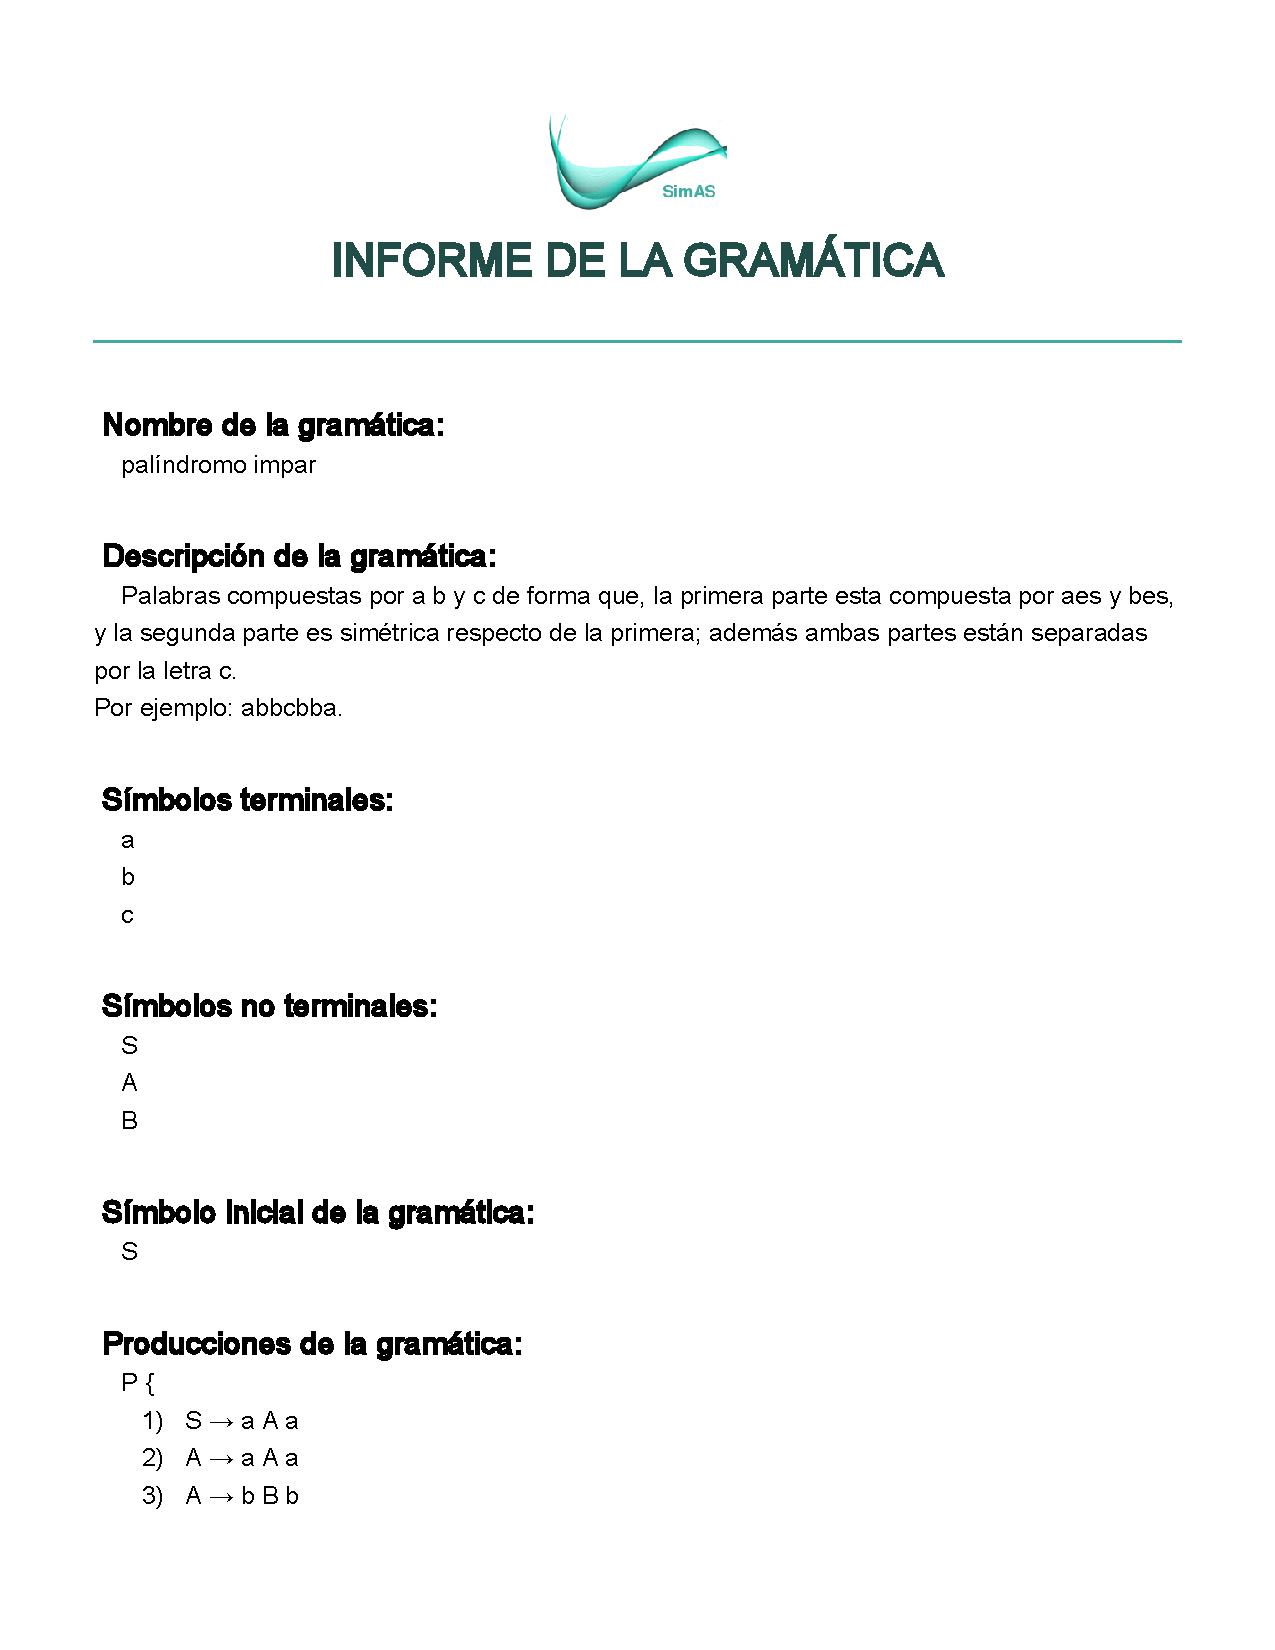
\includepdf[pages=1-2]{documentos/informeGramatica.pdf}


\section{Informe de la simulaci�n}	

 El informe de la simulaci�n de una gram�tica en formato \textit{PDF} se obtiene al realizar la simulaci�n del an�lisis descendente o del an�lisis ascendente sobre una cadena de entrada en la aplicaci�n SimAS. Este informe se guarda directamente en el disco con el nombre de \textit{informeSimulacionDesc.pdf} para el caso del an�lisis descendente y \textit{informeSimulacionAsc.pdf} para el caso del an�lisis ascendente.
 
  A continuaci�n se muestran dos ejemplos del informe de la simulaci�n generado por SimAS, uno del an�lisis sint�ctico descendente y otro del an�lisis sint�ctico ascendente sobre el m�todo \textit{SLR}.
 
  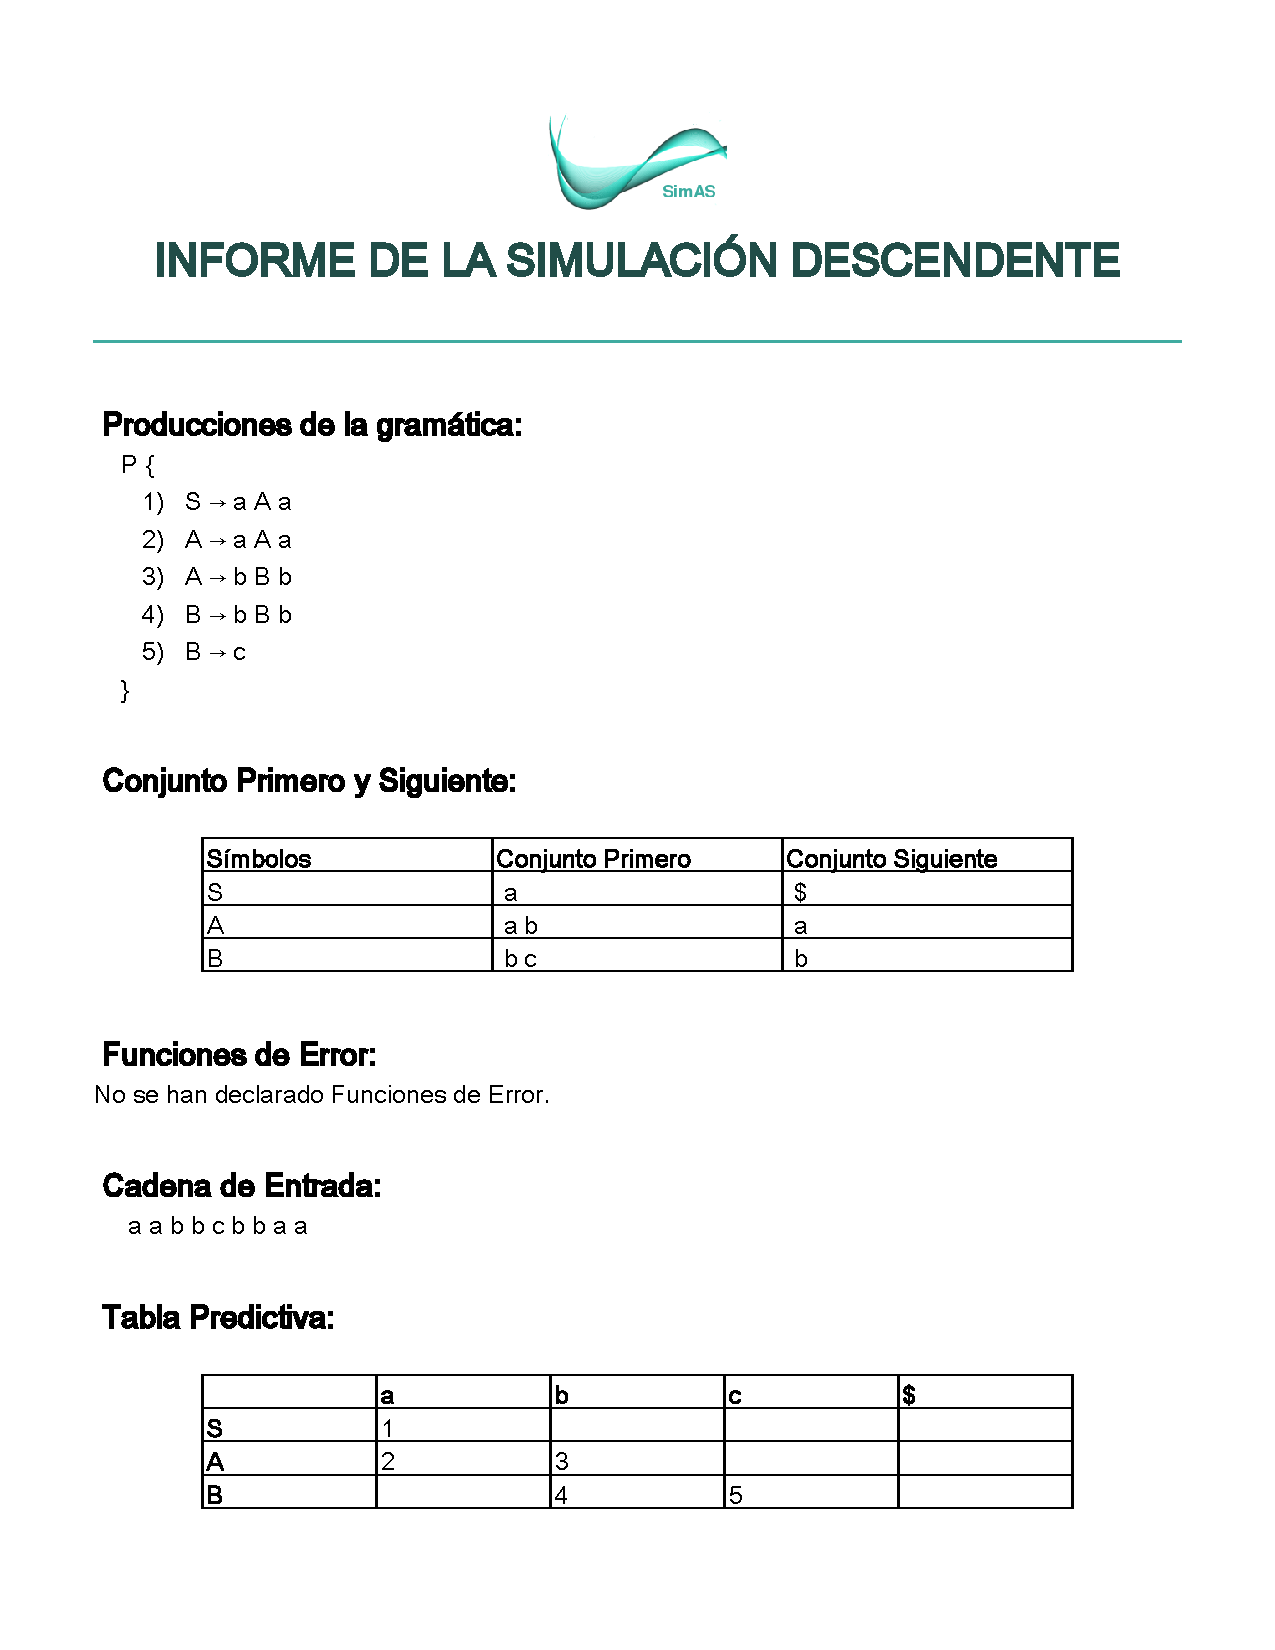
\includepdf[pages=1-2]{documentos/informeSimulacionDesc.pdf}
  
   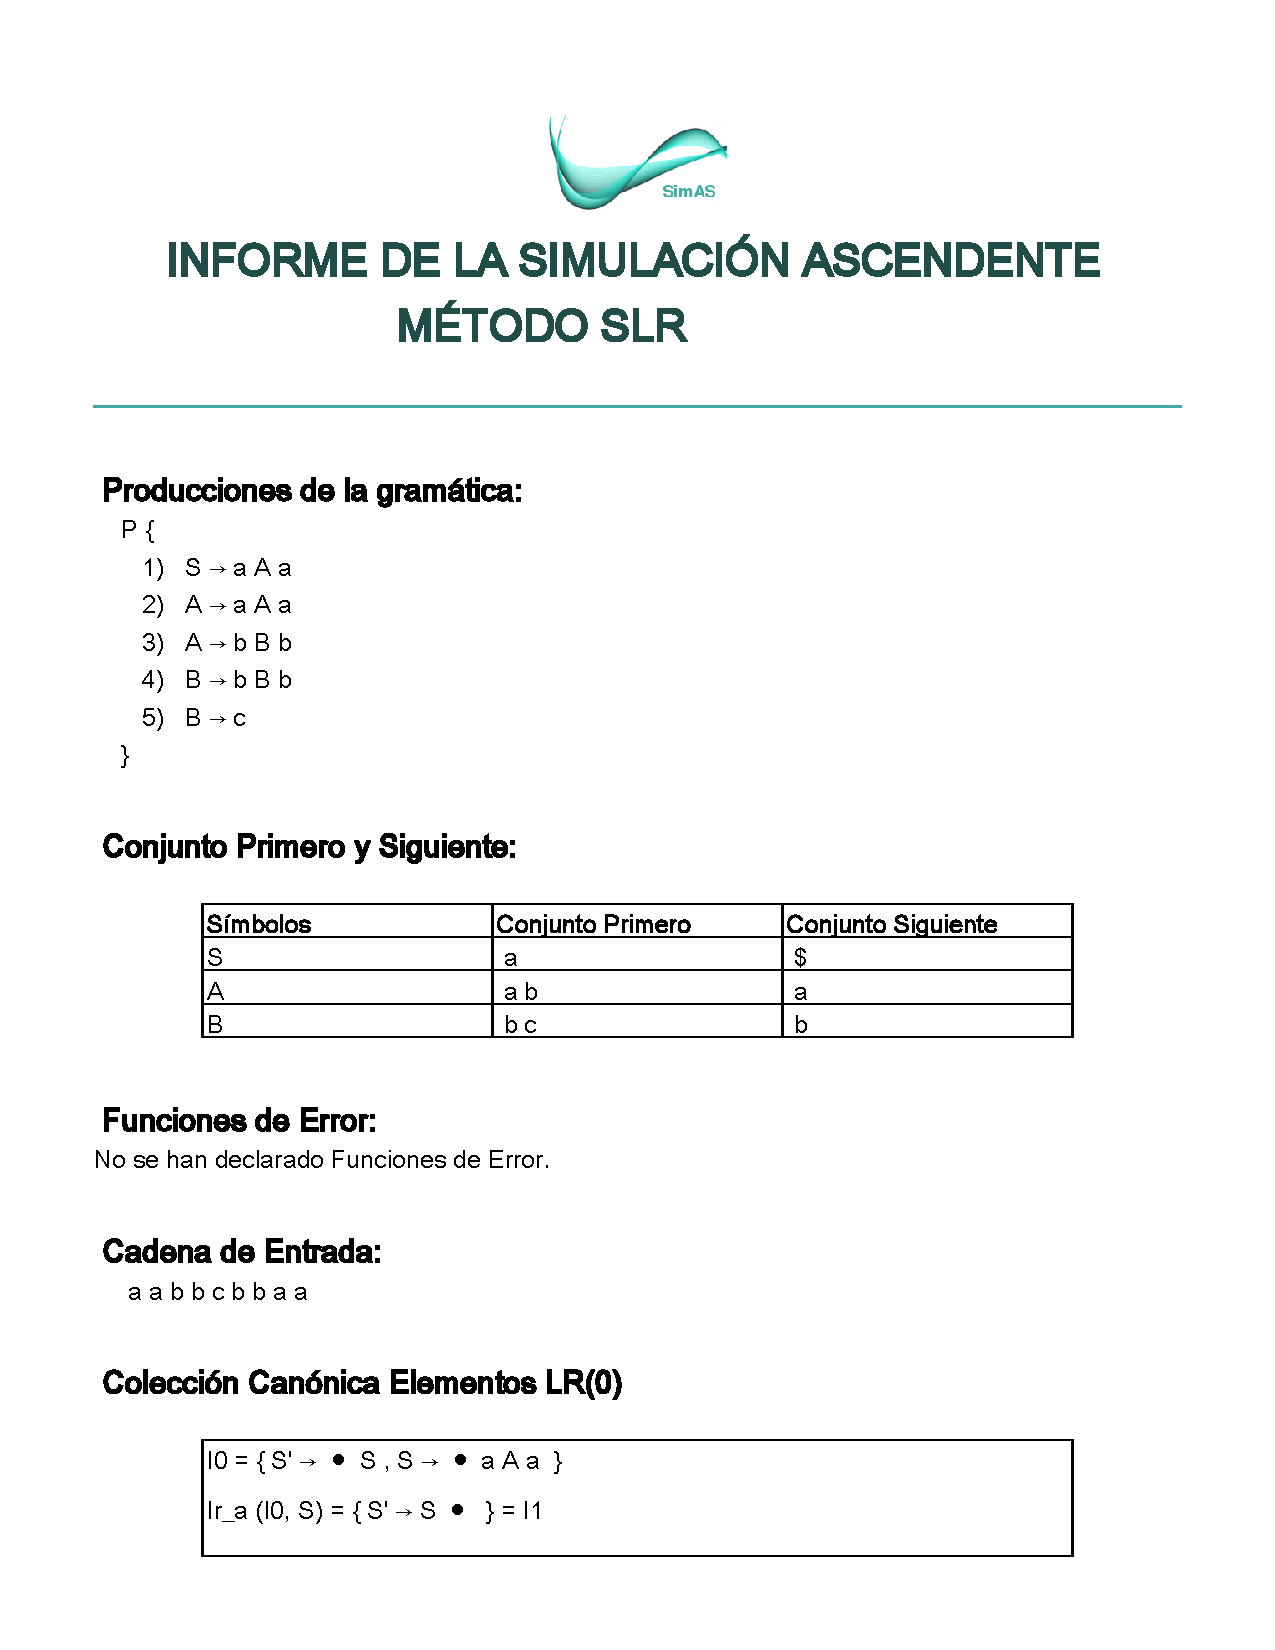
\includepdf[pages=1-4]{documentos/informeSimulacionAsc.pdf}


\section{Documento XML}

 Al crear una gram�tica de contexto libre con la aplicaci�n SimAS, se tiene la opci�n de guardarla, siempre y cuando esta gram�tica sea v�lida, con el objetivo de poder recuperarla en cualquier momento. �sta se guarda en disco en formato \textit{XML} con el nombre que el usuario quiera darle.
 
 A continuaci�n se muestra un ejemplo del documento en formato \textit{XML} que SimAS genera al guardar una gram�tica validada.
 
 \medskip
 \medskip
  \medskip
 \medskip
  \medskip
 \medskip
% \lstinputlisting{documentos/palindromo.xml}

\lstset{language=XML}
\begin{lstlisting}
<?xml version="1.0" encoding="UTF-8"?>
<?xml-stylesheet type="text/xsl" href="gramatica.xsl"?>
<grammar>
	<name>pal�ndromo impar</name>
	<description>Palabras compuestas por a b y c de forma que, la
	     primera parte est� compuesta por aes y bes, y la segunda 
	     parte es sim�trica respecto de la primera; adem�s ambas 
	     partes est�n separadas por la letra c.
         Por ejemplo: abbcbba.</description>
	<non-terminal-symbols>
		<non-terminal>
			<value>S</value>
		</non-terminal>
		<non-terminal>
			<value>A</value>
		</non-terminal>
		<non-terminal>
			<value>B</value>
		</non-terminal>
	</non-terminal-symbols>
	<terminal-symbols>
		<terminal>
			<value>a</value>
		</terminal>
		<terminal>
			<value>b</value>
		</terminal>
		<terminal>
			<value>c</value>
		</terminal>
	</terminal-symbols>
	<init-symbol>S</init-symbol>
	<rule-set>
		<rule>
			<value>S -> a A a </value>
		</rule>
		<rule>
			<value>A -> a A a </value>
		</rule>
		<rule>
			<value>A -> b B b </value>
		</rule>
		<rule>
			<value>B -> b B b </value>
		</rule>
		<rule>
			<value>B -> c </value>
		</rule>
	</rule-set>
</grammar>

\end{lstlisting}



